\section{The split-quintic coefficient}\label{sec:quintic}

The sixteen-node split quintic provides the rank-one application. We specify
the family and calculate its coefficient here. Appendix~\ref{sec:integral-topology}
computes the integral rings, attachments, specialization maps and monodromy
of the same transition; Appendix~\ref{sec:tangent} treats its tangent sheaves.

\subsection{The genuine global family}
Choose independent linear forms $l_1,l_2$ and general quartics $q_1,q_2$
on $\PP^4$, and set
\begin{equation}\label{eq:split-equations}
 \begin{split}
 F_0&=l_1q_2-l_2q_1,\qquad X_0=\{F_0=0\},\\
 Y&=\{ul_1+vl_2=0,\ uq_1+vq_2=0\}
       \subset\PP^4\times\PP^1,\\
 X_t&=\{F_0+tG=0\}.
 \end{split}
\end{equation}
Here $G$ is a quintic nonzero at the sixteen points of
$q_1=q_2=0$ in $\Pi=\{l_1=l_2=0\}$. The precise open conditions
are transversality of the two restricted quartics, smoothness of $X_0$
off $\Pi$, and smoothness of $Y$.

\begin{proposition}\label{prop:split-existence}
These conditions hold on a nonempty open set. The projection $q:Y\to X_0$
is a projective small crepant resolution of exactly sixteen ordinary
nodes. After shrinking the parameter disc, \eqref{eq:split-equations}
is a flat polarized family with trivial relative canonical bundle and
all noncentral fibres smooth. Every node is smoothed to first order.
Both $Y$ and $X_t$ are simply connected.
\end{proposition}
\begin{proof}
The linear system $l_1q_2-l_2q_1$ is the full degree-five ideal of $\Pi$
and is basepoint free off $\Pi$, so Bertini gives smoothness there.
On $\Pi$ its differential is $q_2dl_1-q_1dl_2$. General plane quartics
meet transversely in sixteen points by B\'ezout. At each intersection,
$(l_1,l_2,q_1,q_2)$ are analytic coordinates: the first two are normal
to $\Pi$ and the last two are independent along it. The local equation
is the quadratic determinant, an ordinary double point.

The incidence divisor $ul_1+vl_2=0$ is smooth, including over $\Pi$,
where its normal differential $u\,dl_1+v\,dl_2$ is nonzero. The second
sections $uq_1+vq_2$ form a basepoint-free system there. Bertini gives
smooth $Y$. Projection has a unique kernel line at rank-one matrices
and a whole $\PP^1$ at the sixteen rank-zero matrices. The determinant
coordinates identify its local resolution with
$\OO_{\PP^1}(-1)^{\oplus2}$. Adjunction for the two ample divisor
classes $H+L$ and $4H+L$ gives $K_Y=0$.

The relative hypersurface is flat over a sufficiently small disc.
The condition $G(p_i)\ne0$ gives a simple local smoothing; equivalently
the holomorphic Morse lemma applies to $F_0/G$. Outside the node
neighborhoods, compactness prevents a sequence of critical points from
approaching the smooth central exterior. Thus all sufficiently small
nonzero fibres are smooth. Adjunction gives trivial relative canonical
bundle. Ehresmann's theorem with transverse boundary identifies the
exteriors. Finally integral Lefschetz, twice for $Y$ and once for the
smooth quintic, gives simple connectivity and the integral degree-two
markings used below.
\end{proof}

\begin{figure}[!t]
 \centering
 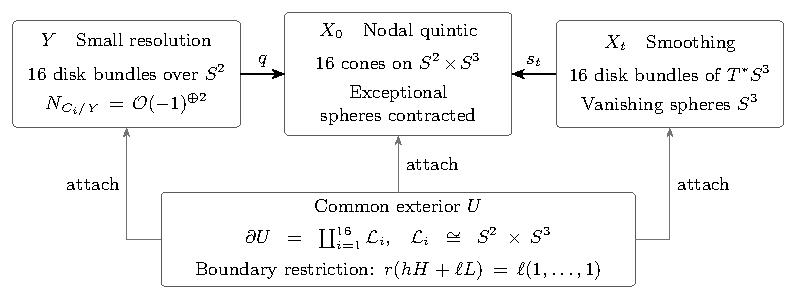
\includegraphics[width=\textwidth]{figures/output/fig01_transition.pdf}
 \caption{The common exterior and its three fillings. The map $q$ is
 algebraic; $s_t$ is the continuous Milnor collapse along the chosen ray.
 The resolution and smoothing cores have real dimensions two and three.
 The same boundary restriction gives the vanishing-cycle relation and
 the periods in the spectral coefficient.}
 \label{fig:transition}
\end{figure}

\subsection{The spectral coefficient and the allowed parameters}
Integral Lefschetz gives $b_2(Y)=2$ and $b_2(X_t)=1$, with generators
$H,L$ and $H$, respectively. The fundamental class of $Y$ in
$\PP^4\times\PP^1$ is $(H+L)(4H+L)$, so
\begin{equation}\label{eq:split-cubic}
 \int_YH^3=5,\qquad \int_YH^2L=4,\qquad L^2=0.
\end{equation}
Every exceptional curve has $(H\cdot C_i,L\cdot C_i)=(0,1)$.
Proposition~\ref{prop:split-existence} therefore verifies the remaining
hypotheses of Theorem~\ref{thm:main}. Taking $D=L$ gives
\[
 M=\frac{4^2}{5}-0=\frac{16}{5},\qquad
 \frac{2\pi\sum_{i=1}^{16}(L\cdot C_i)^2}{M}=10\pi,
\]
which proves Corollary~\ref{cor:quintic} and the spectral assertion of
Theorem~\ref{thm:integrated}.
By Proposition~\ref{prop:restriction-spectrum}, the vector
$(L\cdot C_i)_i=\mathbf1$ in this calculation is the same vector
that generates the kernel of the vanishing-cycle map. The denominator
is the polarized primitive norm from the same integral ring. It is
not an independent local coefficient fitted to the spectrum.

The family has one exceptional-area direction. Arbitrary independent
node parameters are not implied by the number of nodes. Already at
first order, evaluation of quintics at the sixteen planar points has
rank fifteen: the degree-five Hilbert function of a plane $(4,4)$
complete intersection is $\binom72-2\binom32=15$.
Cayley--Bacharach makes the unique evaluation relation nonzero at every
point. The actual pencil selects a compatible vector nonzero at all
nodes. This is sufficient for the fixed-ray theorem and does not
supply uniformity for arbitrary independent smoothing rates.
